\documentclass{beamer}

% Theme
\usetheme{Madrid}
\usecolortheme{default}

% Packages
\usepackage{amsmath,amssymb,amsfonts}
\usepackage{graphicx}
\usepackage{xcolor}
\usepackage{tikz}
\usepackage{tkz-euclide}
\usepackage{array}
\usepackage{multirow}
\usepackage{longtable}
\usepackage{lscape}
\usepackage{listings}
\lstset{
    basicstyle=\ttfamily\small,
    keywordstyle=\color{blue},
    commentstyle=\color{gray},
    stringstyle=\color{red},
    showstringspaces=false,
    breaklines=true
}

% Custom macros
\newcommand{\myvec}[1]{\begin{pmatrix}#1\end{pmatrix}}
\newcommand{\brak}[1]{\left( #1 \right)}
\newcommand{\augvec}[3]{%
  \left(\!\begin{array}{@{}*{#1}{r}|r@{}}#3\end{array}\!\right)
}



% Redefine \vec to bold letters only (no arrow)
\renewcommand{\vec}[1]{\mathbf{#1}}

\title{5.2.22}
\author{EE25BTECH11019 -- Darji Vivek M.}
\date{}

\begin{document}

\begin{frame}
\begin{titlepage}

\end{titlepage}
\end{frame}

\begin{frame}{Question}
Solve for the system of linear equations:
\begin{align*}
    \sqrt{2}x+\sqrt{3}y=0\\
    \sqrt{3}x-\sqrt{8}y=0
\end{align*}
\end{frame}

\begin{frame}{Theoretical Solution}
According to the question,\\
The equation of lines given,
\begin{align}
    \myvec{\sqrt{2}&&\sqrt{3}}\vec{x}=0 \quad \myvec{\sqrt{3}&&-\sqrt{8}}\vec{x}=0
\end{align}
\begin{align}
    \therefore \myvec{\sqrt{2}&&\sqrt{3}\\\sqrt{3}&&-\sqrt{8}}\vec{x}=\myvec{0\\0}
\end{align}
\end{frame}

\begin{frame}{Theoretical Solution}
Forming an augmented matrix,
\[
    \augvec{2}{1}{\sqrt{2} & \sqrt{3} & 0 \\[2pt] \sqrt{3} & -\sqrt{8} & 0}
\]

Upon doing row reduction,
\[
    \augvec{2}{1}{\sqrt{2} & \sqrt{3} & 0 \\[2pt] \sqrt{3} & -\sqrt{8} & 0}
    \xrightarrow{\,R_2 \gets R_2 - \tfrac{\sqrt{3}}{\sqrt{2}} R_1\,}
    \augvec{2}{1}{\sqrt{2} & \sqrt{3} & 0 \\[2pt] 0 & -\sqrt{8}-\tfrac{3}{\sqrt{2}} & 0}
\]

\[
    \xrightarrow{\,R_1 \gets R_1 + 0\times R_2\,}
    \augvec{2}{1}{\sqrt{2} & \sqrt{3} & 0 \\[2pt] 0 & -\sqrt{8}-\tfrac{3}{\sqrt{2}} & 0}
\]

\begin{align}
    \implies \vec{x}=\myvec{0\\0}
\end{align}
\end{frame}



\begin{frame}[fragile]{C Code: parallel\_funcs.c}
\begin{lstlisting}
#include <math.h>
// Function to find the intersection of two lines
// Line 1: a1*x + b1*y = c1
// Line 2: a2*x + b2*y = c2
// result[0] = x, result[1] = y
void intersection(double a1, double b1, double c1,
                  double a2, double b2, double c2,
                  double *result)
{
    double det = a1*b2 - a2*b1;
    if (fabs(det) < 1e-9) {
        // Lines are parallel or coincident
        result[0] = NAN;
        result[1] = NAN;
        return;
    }
    result[0] = (c1*b2 - c2*b1) / det;
    result[1] = (a1*c2 - a2*c1) / det;
}
\end{lstlisting}
\end{frame}

\begin{frame}[fragile]{Python: Plotting Lines}
\begin{lstlisting}[language=Python, basicstyle=\ttfamily\scriptsize, keywordstyle=\color{blue}]
import ctypes
import numpy as np
import matplotlib.pyplot as plt

# Load the C library
lib = ctypes.CDLL('./10.so')

# Define argument and return types
lib.intersection.argtypes = [ctypes.c_double, ctypes.c_double, ctypes.c_double,
                             ctypes.c_double, ctypes.c_double, ctypes.c_double,
                             ctypes.POINTER(ctypes.c_double)]

# Prepare variables
a1, b1, c1 = np.sqrt(2), np.sqrt(3), 0
a2, b2, c2 = np.sqrt(3), -np.sqrt(8), 0

# Result array
res = (ctypes.c_double * 2)()
lib.intersection(a1, b1, c1, a2, b2, c2, res)
\end{lstlisting}
\end{frame}

\begin{frame}[fragile]{Python: Plotting Lines}
\begin{lstlisting}[language=Python, basicstyle=\ttfamily\scriptsize, keywordstyle=\color{blue}]

x_inter, y_inter = res[0], res[1]
print(f"Intersection point: ({x_inter:.2f}, {y_inter:.2f})")

# Generate line points
x = np.linspace(-5, 5, 100)
y1 = (-a1 * x + c1) / b1
y2 = (-a2 * x + c2) / b2

# Plot lines
plt.plot(x, y1, label=r'$\sqrt{2}x + \sqrt{3}y = 0$')
plt.plot(x, y2, label=r'$\sqrt{3}x - \sqrt{8}y = 0$')
plt.scatter(x_inter, y_inter, color='red', label='Intersection Point (0,0)')
plt.axhline(0, color='black', linewidth=0.5)
plt.axvline(0, color='black', linewidth=0.5)
plt.xlabel('x')
plt.ylabel('y')
plt.title('Intersection of Two Lines')
plt.legend()
plt.grid(True)
plt.show()
\end{lstlisting}
\end{frame}

\begin{frame}{Pyhton plot}
\begin{figure}[h!]
    \centering
    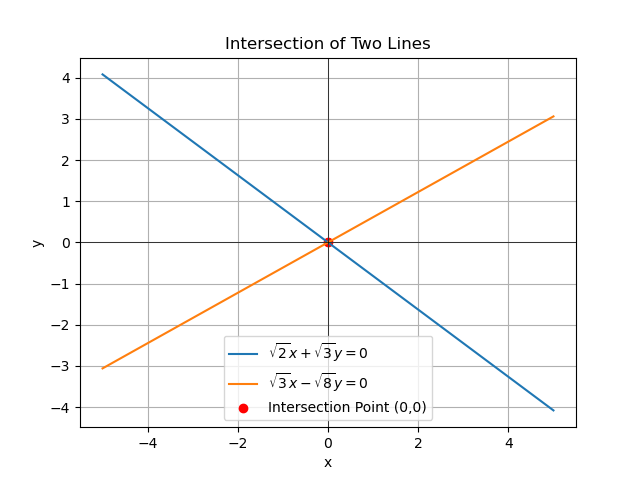
\includegraphics[width=0.75\textwidth]{figs/10.png}
    \caption{parallel lines}
    \label{fig:example_image}
\end{figure}
\end{frame}

\end{document}